\chapter{Aminas e compostos nitrogenados}\label{ch:b2:amines}

O peixe que já não está fresco cheira a trimetilamina, uma pequena amina
volátil. Umas gotas de limão eliminam o cheiro: o ácido protona a amina, e o
íon amônio formado, sendo um íon, não consegue evaporar. O par não ligante do
nitrogênio faz das aminas bases e nucleófilos; ligado a uma carbonila, ele dá
\omterm{def:b2:amines:imine}{iminas}, pelas quais as proteínas realizam sua química e os químicos fabricam
aminas; e, em um anel \omterm{def:b2:huckel:aromatic}{aromático}, ele abre, por meio dos sais de diazônio, o
caminho para os corantes azo que coloriram o século XIX.

\begin{recall}
O volume do 1.º ano: ácidos e bases de Brønsted, $\mathrm pK_a$ e diagramas de
predominância, nucleófilos e a substituição bimolecular, hemiacetais e
acetais, doadores de hidreto, compostos organomagnesianos, a classe de um
carbono. \Cref{ch:b2:aromatic-substitution}: a nitração, a redução dos
nitroarenos. O volume escolar: aminas e amidas.
\end{recall}

\begin{omfigure}
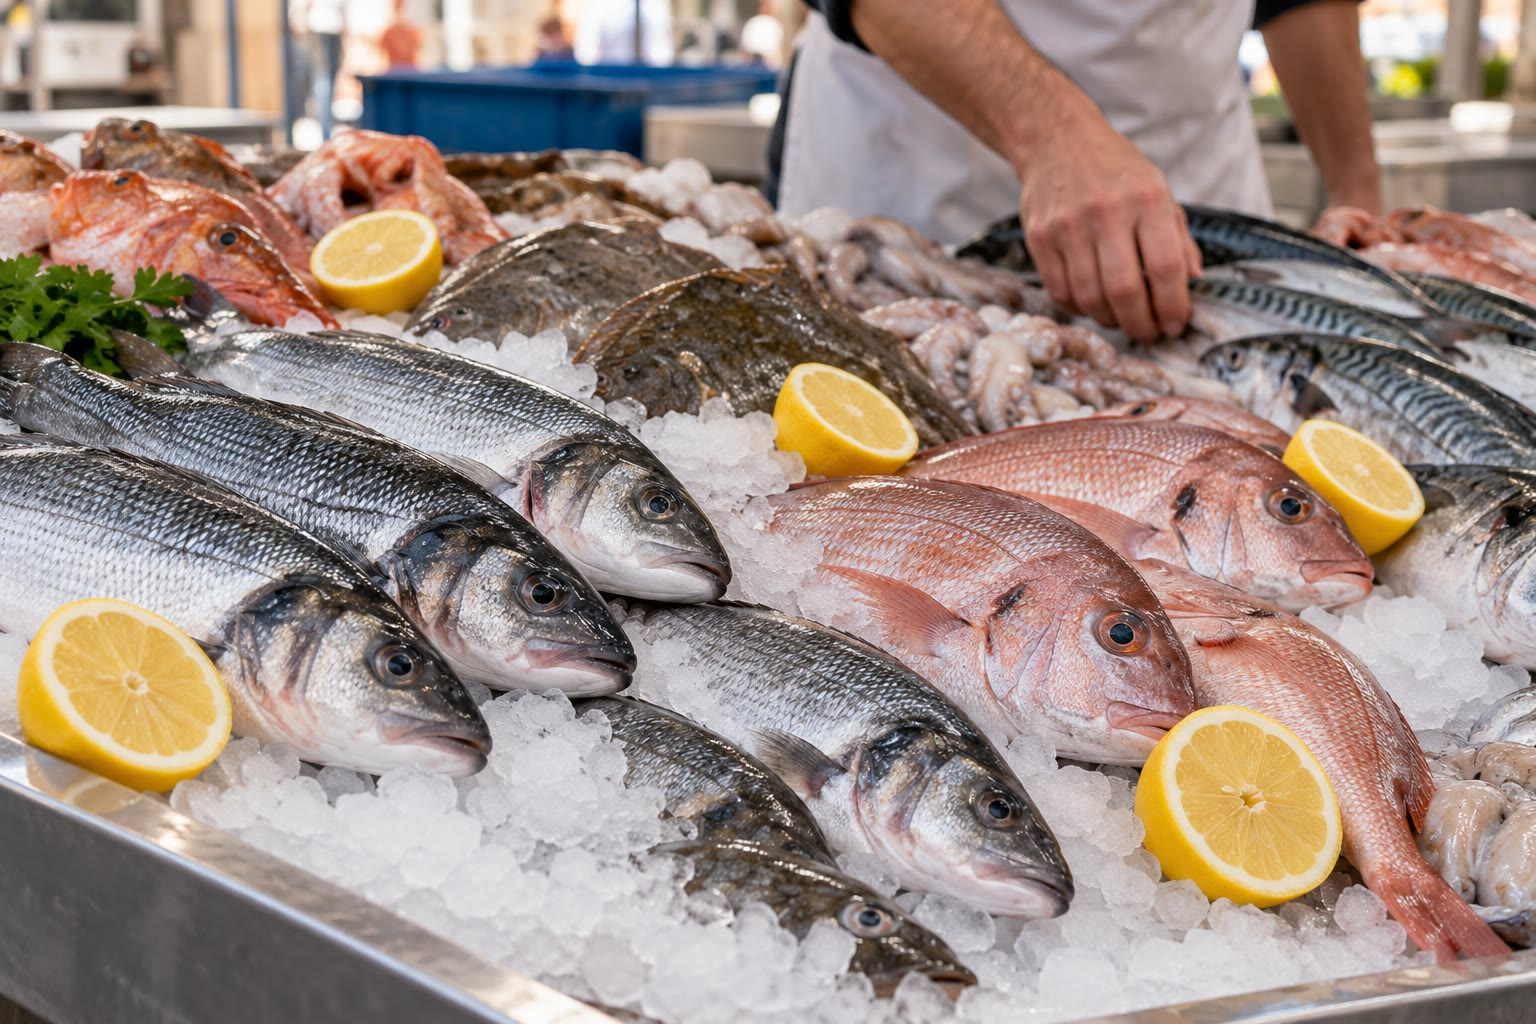
\includegraphics[width=0.6\linewidth]{images/book3/ai/b2-23-fish-stall.jpg}

{\small Uma banca de peixe: limões cortados ao meio são colocados entre os
peixes. Seu ácido transforma a trimetilamina do peixe em seu íon amônio não
volátil.}
\end{omfigure}

\section{Estrutura e basicidade}

\begin{definition}[Classes das aminas]\label{def:b2:amines:class}
Uma amina é uma \emph{amina primária}\index{amina primaria@amina primária} \ce{RNH2}, uma \emph{amina secundária}
\index{amina secundaria@amina secundária} \ce{R2NH} ou uma \emph{amina terciária}\index{amina terciaria@amina terciária}
\ce{R3N} conforme o número de grupos carbonados ligados ao nitrogênio. Um
\emph{íon amônio quaternário}\index{ion amonio quaternario@íon amônio quaternário} \ce{R4N+} tem quatro, e nenhum par não
ligante.
\end{definition}

O nitrogênio de uma amina é aproximadamente tetraédrico, com o par não ligante
ocupando a quarta posição. Uma \omterm{def:b2:amines:class}{amina terciária} com três grupos diferentes é
quiral em princípio, mas não pode ser resolvida: a molécula se inverte
passando por um arranjo plano, como um guarda-chuva ao vento, bilhões de vezes
por segundo à temperatura ambiente.

\begin{proposition}[Basicidade]\label{prop:b2:amines:basicity}
Em água, as alquilaminas são bases mais fortes que a amônia ($\mathrm pK_a$ de
seus íons amônio perto de 10 a 11, contra 9.26), as arilaminas muito mais
fracas (anilínio 4.60), e as amidas quase nada básicas (etanamida protonada,
cerca de $-0.6$).
\end{proposition}

\begin{proof}[Raciocínio]
Os grupos alquila empurram densidade eletrônica para o nitrogênio (efeito
indutivo) e estabilizam a carga positiva do íon amônio. Em água, a solvatação
por ligações de hidrogênio também importa: um íon com mais ligações \ce{N-H} é
mais bem solvatado; é por isso que o trimetilamônio (9.80) é um ácido mais
fraco que o amônio, mas mais forte que o dimetilamônio (10.73). Na anilina, o
par não ligante está deslocalizado no anel e se perde na protonação; em uma
amida, ele está deslocalizado no oxigênio da carbonila, e a protonação ocorre,
fracamente, no oxigênio.
% ledger: kb:NH3, pka:methylammonium, pka:dimethylammonium, pka:trimethylammonium, pka:anilinium, pka:ethanamideH
\end{proof}

\begin{omfigure}
\begin{tikzpicture}[font=\small, x=0.85cm]
  \draw[->, thick] (-1.5,0) -- (11.8,0) node[below right] {$\mathrm pK_a$};
  \foreach \x in {0,2,4,6,8,10} \draw (\x,0.1) -- (\x,-0.1) node[below, font=\scriptsize] {\x};
  \foreach \x/\l in {-0.6/{\ce{CH3CONH3+}}, 4.60/{\ce{C6H5NH3+}}} {
    \draw[omDef, thick] (\x,0) -- (\x,0.5);
    \node[font=\scriptsize, anchor=south] at (\x,0.5) {\l};
  }
  \foreach \x/\l/\y/\h in {9.26/{\ce{NH4+} (9.26)}/1.95/1.2, 9.80/{\ce{(CH3)3NH+} (9.80)}/1.45/0.85, 10.66/{\ce{CH3NH3+} (10.66)}/0.95/0.5, 10.73/{\ce{(CH3)2NH2+} (10.73)}/0.45/0.25} {
    \draw[omDef, thick] (\x,0) -- (\x,\h);
    \draw[black!40] (\x,\h) -- (12.2,\y);
    \node[font=\scriptsize, anchor=west] at (12.2,\y) {\l};
  }
  \node[font=\scriptsize, anchor=north west] at (-1.4,-0.5) {bases mais fracas};
  \node[font=\scriptsize, anchor=north east] at (11.7,-0.5) {bases mais fortes};
\end{tikzpicture}

{\small $\mathrm pK_a$ dos ácidos conjugados de algumas bases nitrogenadas a
\qty{25}{\degreeCelsius}: quanto mais alto, mais forte a base.}
% ledger: kb:NH3, pka:methylammonium, pka:dimethylammonium, pka:trimethylammonium, pka:anilinium, pka:ethanamideH
\end{omfigure}

\section{As aminas como nucleófilos}

As aminas atacam os haloalcanos por substituição bimolecular. O produto, uma
amina mais substituída, é pelo menos tão nucleofílico quanto a de partida e
compete pelo haloalcano: a alquilação da amônia dá uma mistura de \omterm{def:b2:amines:class}{aminas
primárias}, secundárias e terciárias e do sal quaternário.

\begin{proposition}[Polialquilação]\label{prop:b2:amines:polyalkylation}
A alquilação direta da amônia ou de uma \omterm{def:b2:amines:class}{amina primária} dá misturas; só a
alquilação exaustiva até o sal de amônio quaternário é limpa.
\end{proposition}

\begin{proof}[Raciocínio]
Cada alquilação deixa um par não ligante em um nitrogênio tornado mais rico em
elétrons pelo novo grupo alquila; o produto reage com o haloalcano restante a
uma velocidade comparável. Só quando o nitrogênio não tem mais par não ligante,
em \ce{R4N+}, a sequência para.
\end{proof}

As \omterm{def:b2:amines:class}{aminas primárias} isentas de seus parentes sobrealquilados são obtidas
indiretamente: pela via de Gabriel (alquilação do nitrogênio da ftalimida, que
tem um único hidrogênio ácido, seguida da liberação da amina), por redução de
uma \omterm{def:b2:amines:nitrile}{nitrila}, de uma amida ou de um composto nitro, ou por \omterm{def:b2:amines:reductive-amination}{aminação redutiva}
(abaixo).

\section{Iminas e enaminas}

\begin{definition}[Adição nucleofílica]\label{def:b2:amines:nucleophilic-addition}
Uma \emph{adição nucleofílica}\index{adicao nucleofilica@adição nucleofílica} a um grupo carbonila é o ataque
de um nucleófilo ao carbono carbonílico, que se torna tetraédrico, enquanto a
ligação $\pi$ \ce{C=O} se torna um par não ligante no oxigênio.
\end{definition}

\begin{definition}[Hemiaminais, iminas e enaminas]\label{def:b2:amines:imine}
Uma \omterm{def:b2:amines:class}{amina primária} se adiciona a um aldeído ou a uma cetona dando um
\emph{hemiaminal}\index{hemiaminal} (um carbono que leva \ce{OH} e \ce{NHR}); sua
desidratação dá uma \emph{imina}\index{imina}
$\mathrm{R_2C{=}NR'}$. Uma \omterm{def:b2:amines:class}{amina secundária}, que não pode formar uma imina
neutra, dá após desidratação uma
\emph{enamina}\index{enamina} $\mathrm{R_2C{=}CR{-}NR'_2}$, com a ligação dupla
passando para o carbono vizinho.
\end{definition}

\begin{omfigure}
\setchemfig{atom sep=1.9em}
\schemestart
\chemfig{R_2C=O} \+ \chemfig{H_2N-R'}
\arrow{<=>}
\chemfig{R_2C(-[2]OH)-NH-R'}
\arrow{<=>[\ce{H+}][$-$ \ce{H2O}]}
\chemfig{R_2C=N-R'}
\schemestop
\par\vspace{6pt}

{\small Formação de uma \omterm{def:b2:amines:imine}{imina}: a \omterm{def:b2:amines:nucleophilic-addition}{adição nucleofílica} da amina à carbonila dá o
\omterm{def:b2:amines:imine}{hemiaminal}; a catálise ácida transforma seu \ce{OH} em grupo de saída
(\ce{-OH2+}), a água sai e o par não ligante do nitrogênio forma a ligação
dupla \ce{C=N}. Todas as etapas são reversíveis: a água em excesso hidrolisa de
volta a \omterm{def:b2:amines:imine}{imina}.}
\end{omfigure}

\begin{proposition}[pH ótimo]\label{prop:b2:amines:imine-ph}
As \omterm{def:b2:amines:imine}{iminas} se formam mais depressa em solução levemente ácida, perto de pH 4 a 5.
\end{proposition}

\begin{proof}[Raciocínio]
A primeira etapa precisa da amina livre (de seu par não ligante); um meio
ácido demais protona a amina ($\mathrm pK_a$ cerca de 10) e elimina o
nucleófilo. A desidratação precisa de ácido para protonar o grupo hidroxila; em
pH alto, ela é lenta. A velocidade, produto das duas necessidades, é máxima
entre os dois extremos.
\end{proof}

\begin{definition}[Aminação redutiva]\label{def:b2:amines:reductive-amination}
Uma \emph{aminação redutiva}\index{aminacao redutiva@aminação redutiva} converte um composto carbonílico e
uma amina em uma amina mais substituída, formando a \omterm{def:b2:amines:imine}{imina} (ou o íon imínio) e
reduzindo-a no mesmo frasco, em geral com cianoboro-hidreto de sódio
\ce{NaBH3CN}.
\end{definition}

\begin{proposition}[Seletividade da aminação redutiva]\label{prop:b2:amines:reductive-amination}
Em pH perto de 6, o \ce{NaBH3CN} reduz o íon imínio muito mais depressa que o
composto carbonílico, de modo que a amina se forma sem que o aldeído ou a
cetona sejam reduzidos a álcool.
\end{proposition}

\begin{proof}[Raciocínio]
O grupo ciano faz de \ce{BH3CN-} um doador de hidreto fraco, fraco demais para
uma carbonila neutra, mas suficiente para um íon imínio protonado, carregado
positivamente, um eletrófilo muito melhor.
\end{proof}

\section{Os sais de diazônio}

\begin{definition}[Química dos diazônios]\label{def:b2:amines:diazonium}
Um \emph{íon diazônio}\index{ion diazonio@íon diazônio} é um cátion \ce{R-N+#N}. A \emph{diazotação}\index{diazotacao@diazotação}
converte uma amina \omterm{def:b2:huckel:aromatic}{aromática} primária em um sal de arildiazônio com nitrito de
sódio e um ácido forte a 0--\qty{5}{\degreeCelsius}. Em uma \emph{reação de
Sandmeyer}\index{reacao de Sandmeyer@reação de Sandmeyer}, um sal de cobre(I)
(\ce{CuCl}, \ce{CuBr}, \ce{CuCN}) substitui o grupo diazônio por Cl, Br ou CN, com
perda de dinitrogênio. Em um \emph{acoplamento azo}\index{acoplamento azo}, o íon diazônio,
um eletrófilo fraco, ataca um anel \omterm{def:b2:huckel:aromatic}{aromático} ativado, dando um composto azo
$\mathrm{Ar{-}N{=}N{-}Ar'}$.
\end{definition}

\begin{proposition}[Estabilidade dos íons diazônio]\label{prop:b2:amines:diazonium}
Os sais de arildiazônio podem ser conservados em solução aquosa fria e
usados; os íons alquildiazônio perdem dinitrogênio de imediato.
\end{proposition}

\begin{proof}[Raciocínio]
O dinitrogênio é um excelente grupo de saída (uma molécula muito estável, um
grande ganho de entropia). Para um grupo alquila, a perda de \ce{N2} deixa um
carbocátion, ou o íon é atacado diretamente pela água: ele não sobrevive. Um
cátion arila é muito instável (um orbital $\sigma$ vazio no plano do anel, não
estabilizado pelo sistema $\pi$), e a ligação \ce{C-N} do íon arildiazônio é
reforçada pela conjugação com o anel: a baixa temperatura, ele persiste;
aquecido, ele se decompõe, com a água substituindo o grupo diazônio por \ce{OH}.
\end{proof}

\begin{omfigure}
\begin{tikzpicture}[font=\small, >={Stealth}]
  \node[cyclenode] (d) at (0,0) {\ce{Ar-N2+}};
  \foreach \a/\t/\c in {90/{\ce{Ar-Cl}}/{\ce{CuCl}}, 150/{\ce{Ar-Br}}/{\ce{CuBr}}, 210/{\ce{Ar-CN}}/{\ce{CuCN}},
                        270/{\ce{Ar-OH}}/{\ce{H2O}, a quente}, 330/{\ce{Ar-H}}/{\ce{H3PO2}}, 30/{$\mathrm{Ar{-}N{=}N{-}Ar'}$}/{\ce{ArH} ativado}} {
    \node[cyclenode] (p\a) at (\a:2.6) {\t};
    \draw[->, thick] (d) -- (p\a) node[midway, font=\scriptsize, fill=white, inner sep=1pt] {\c};
  }
\end{tikzpicture}

{\small Reações de um sal de arildiazônio. O grupo \ce{N2+} é substituído por
halogênio ou cianeto (Sandmeyer, sais de cobre(I)), por \ce{OH} (água quente)
ou por H (ácido hipofosforoso), ou é conservado em um \omterm{def:b2:amines:diazonium}{acoplamento azo}.}
\end{omfigure}

\begin{method}[Vias que passam por um sal de diazônio]\label{met:b2:amines:diazonium-routes}
\begin{enumerate}
  \item Use o grupo amino (forte \omterm{def:b2:aromatic-substitution:directing}{orientador orto/para}) para posicionar outros
        grupos e depois converta-o por meio do sal de diazônio.
  \item Substitua-o por H para obter padrões que a substituição direta não
        consegue dar (o 1,3,5-tribromobenzeno a partir da anilina).
  \item Substitua-o por CN e depois hidrolise a ácido carboxílico: um caminho
        para um \ce{-COOH} em um anel.
\end{enumerate}
\end{method}

\begin{method}[Preparar uma amina]\label{met:b2:amines:make-amine}
\begin{enumerate}
  \item \omterm{def:b2:amines:class}{Amina primária} em uma cadeia alquila: via de Gabriel, ou redução de
        uma \omterm{def:b2:amines:nitrile}{nitrila} (um carbono a mais que o haloalcano usado para prepará-la)
        ou de uma amida.
  \item \omterm{def:b2:amines:class}{Amina secundária} ou terciária: \omterm{def:b2:amines:reductive-amination}{aminação redutiva} do composto
        carbonílico certo com a amina certa.
  \item Amina \omterm{def:b2:huckel:aromatic}{aromática}: nitração e depois redução (ferro ou estanho com
        ácido, ou \omterm{def:b2:alkene-redox:hydrogenation}{hidrogenação catalítica}).
\end{enumerate}
\end{method}

\section{As nitrilas}

\begin{definition}[Nitrila]\label{def:b2:amines:nitrile}
Uma \emph{nitrila}\index{nitrila} é um composto \ce{R-C#N}, obtido por substituição de
um haloalcano pelo cianeto ou por uma \omterm{def:b2:amines:diazonium}{reação de Sandmeyer}.
\end{definition}

\begin{proposition}[Reações das nitrilas]\label{prop:b2:amines:nitrile}
Uma \omterm{def:b2:amines:nitrile}{nitrila} é hidrolisada, em meio ácido ou básico, à amida e depois ao ácido
carboxílico; ela é reduzida pelo hidreto de lítio e alumínio à \omterm{def:b2:amines:class}{amina primária}
\ce{RCH2NH2}; um composto organomagnesiano se adiciona a ela uma única vez, e a
hidrólise da \omterm{def:b2:amines:imine}{imina} formada dá uma cetona.
\end{proposition}

\begin{proof}[Raciocínio]
O carbono da \omterm{def:b2:amines:nitrile}{nitrila} é eletrofílico, como um carbono carbonílico: a água
(ativada por ácido, ou como hidróxido) se adiciona a ele, dando após
tautomeria uma amida, cuja hidrólise é tratada no
\cref{ch:b2:acyl-substitution}. O hidreto se adiciona duas vezes. Um composto
organomagnesiano se adiciona uma vez, dando um ânion \omterm{def:b2:amines:imine}{imina} que não reage mais;
a água então hidrolisa a \omterm{def:b2:amines:imine}{imina} à cetona.
\end{proof}

\begin{safety}{\ghs[5mm]{GHS03}\,\ghs[5mm]{GHS06}\,\ghs[5mm]{GHS08}\,\ghs[5mm]{GHS09}}
A anilina e a \textit{N},\textit{N}-dimetilanilina são tóxicas por contato com a
pele; o nitrito de sódio é tóxico e oxidante; o cianoboro-hidreto de sódio
libera cianeto de hidrogênio em meio ácido e deve ser usado na capela. Os sais
de diazônio secos podem explodir: eles são sempre mantidos frios, em solução, e
usados de imediato.
% ledger: ghs:aniline, ghs:dimethylaniline, ghs:NaNO2, ghs:NaBH3CN, ghs:sulfanilic-acid
\end{safety}

\section{Exercícios}

\begin{exercise}[$\star$]\label{exo:b2:amines:1}
Dê a classe de: propan-1-amina, \textit{N}-metiletanamina, trietilamina,
cloreto de tetrametilamônio, anilina.
\end{exercise}

\begin{exercise}[$\star$]\label{exo:b2:amines:2}
Ordene por basicidade crescente: amônia, metilamina, anilina, etanamida.
\end{exercise}

\begin{exercise}[$\star$]\label{exo:b2:amines:3}
Dê a \omterm{def:b2:amines:imine}{imina} formada a partir da ciclo-hexanona e da metilamina, e as condições.
\end{exercise}

\begin{exercise}[$\star$]\label{exo:b2:amines:4}
A partir do cloreto de benzenodiazônio, dê os produtos com \ce{CuBr}, \ce{CuCN},
água quente e fenol em meio básico.
\end{exercise}

\begin{exercise}[$\star\star$]\label{exo:b2:amines:5}
Que forma da trimetilamina predomina a pH 7, e em que razão? Explique o limão e
como uma amina pode ser extraída de um solvente orgânico para a água.
\end{exercise}

\begin{exercise}[$\star\star$]\label{exo:b2:amines:6}
Dê a \omterm{def:b2:amines:imine}{enamina} formada a partir da ciclo-hexanona e da pirrolidina, e explique
por que uma \omterm{def:b2:amines:class}{amina secundária} não pode dar uma \omterm{def:b2:amines:imine}{imina}.
\end{exercise}

\begin{exercise}[$\star\star$]\label{exo:b2:amines:7}
Prepare a \textit{N}-benzilpropan-2-amina \ce{C6H5CH2NHCH(CH3)2} por \omterm{def:b2:amines:reductive-amination}{aminação
redutiva}: dê dois pares possíveis de reagentes.
\end{exercise}

\begin{exercise}[$\star\star$]\label{exo:b2:amines:8}
A benzonitrila reage com brometo de etilmagnésio e depois com ácido aquoso. Dê o produto.
\end{exercise}

\begin{exercise}[$\star\star$]\label{exo:b2:amines:9}
Escreva a síntese de Gabriel da hexan-1-amina e explique por que ela não dá \omterm{def:b2:amines:class}{amina secundária}.
\end{exercise}

\begin{exercise}[$\star\star\star$]\label{exo:b2:amines:10}
Prepare o 1,3,5-tribromobenzeno a partir da anilina.
\end{exercise}

\begin{exercise}[$\star\star\star$]\label{exo:b2:amines:11}
Planeje um corante azo a partir da 4-nitroanilina e do fenol: escreva a
\omterm{def:b2:amines:diazonium}{diazotação}, o acoplamento (posição e pH) e o produto.
\end{exercise}

\begin{exercise}[$\star\star\star$]\label{exo:b2:amines:12}
O hidróxido de amônio quaternário da \textit{N},\textit{N}-dimetilbutan-2-amina,
aquecido, dá sobretudo but-1-eno. Explique essa orientação de Hofmann, oposta
à regra de Zaitsev do volume do 1.º ano.
\end{exercise}

\section{Problema: Preparar o alaranjado de metila}

\begin{problem}[{Problema de fim de semana --- o ácido sulfanílico e sua \omterm{def:b2:amines:diazonium}{diazotação}, o
\omterm{def:b2:amines:diazonium}{acoplamento azo} com a \textit{N},\textit{N}-dimetilanilina, o alaranjado de
metila como indicador e o rendimento}]
\label{pb:b2:amines:1}
Dados: ácido sulfanílico (ácido 4-aminobenzenossulfônico) \ce{C6H7NO3S}; alaranjado
de metila, o sal de sódio \ce{C14H14N3NaO3S}; $\mathrm pK_a$ da forma ácida do
alaranjado de metila 3.47. Massas molares (\unit{g/mol}): C 12.011, H 1.008,
N 14.007, O 15.999, Na 22.990, S 32.06. Ensaio (dados do exercício):
\qty{5.00}{g} de ácido sulfanílico, rendimento de 80~\%.
% ledger: pka:methylorange, aw:C, aw:H, aw:N, aw:O, aw:Na, aw:S, ghs:sulfanilic-acid, ghs:NaNO2

\medskip
\noindent\textbf{Parte I --- O ácido sulfanílico e a \omterm{def:b2:amines:diazonium}{diazotação}.}
\begin{enumerate}
  \item O ácido sulfanílico existe como zwitteríon. Desenhe-o.
  \item Por que ele é dissolvido primeiro em solução de carbonato de sódio?
  \item Escreva a formação do ácido nitroso a partir do nitrito de sódio e do ácido clorídrico.
  \item Escreva a \omterm{def:b2:amines:diazonium}{diazotação} do íon 4-sulfonatoanilínio.
  \item Por que a reação é conduzida a 0--\qty{5}{\degreeCelsius}?
  \item Que quantidade de nitrito de sódio é necessária para \qty{5.00}{g} de ácido sulfanílico?
  \item Por que se verifica e se destrói um leve excesso de nitrito?
\end{enumerate}

\medskip
\noindent\textbf{Parte II --- O acoplamento.}
\begin{enumerate}[resume]
  \item Por que a \textit{N},\textit{N}-dimetilanilina é um bom parceiro?
  \item Em que posição de seu anel o \omterm{def:b2:amines:diazonium}{íon diazônio} ataca, e por quê?
  \item Escreva o produto (como sulfonato).
  \item Por que o acoplamento é feito em solução fracamente ácida, e não fortemente ácida?
  \item Por que a solução deve depois ser tornada básica para precipitar o sal de sódio?
  \item Por que o \omterm{def:b2:amines:diazonium}{íon diazônio} é um eletrófilo fraco, que só reage com anéis ativados?
\end{enumerate}

\medskip
\noindent\textbf{Parte III --- Um indicador.}
\begin{enumerate}[resume]
  \item De que cor é o alaranjado de metila em meio básico, e em meio ácido?
  \item Onde ele recebe um próton?
  \item Em que faixa de pH sua cor muda?
  \item Por que o sistema conjugado estendido dá uma cor visível?
  \item Por que a protonação desloca a absorção?
\end{enumerate}

\medskip
\noindent\textbf{Parte IV --- O rendimento.}
\begin{enumerate}[resume]
  \item Calcule a massa molar do ácido sulfanílico.
  \item Calcule a do alaranjado de metila (sal de sódio).
  \item Calcule a quantidade de ácido sulfanílico usada.
  \item Calcule a massa teórica de alaranjado de metila.
  \item Que perdas explicam um rendimento inferior a 100~\%?
  \item Dê a massa de alaranjado de metila obtida a partir de \qty{5.00}{g} de
        ácido sulfanílico com 80~\% de rendimento.
\end{enumerate}
\end{problem}
